%
% Tesi D.S.I. - modello preso da
% Stanford University PhD thesis style -- modifications to the report style
%
%%%%%%%%%%%%%%%%%%%%%%%%%%%%%%%%%%%%%%%%%%%%%%%%%%%%%%%%%%%%%%%%%%%%%%%%%%%
%                                                                         %
%			TESI DOTTORATO                                                   %
%			______________                                                   %
%                                                                         %
%			AUTORE: Elena Pagani                                             %
%                                                                         %
%			Ultima revisione: 7.X.1998                                       %
%           correzioni atrent                                             %
%%%%%%%%%%%%%%%%%%%%%%%%%%%%%%%%%%%%%%%%%%%%%%%%%%%%%%%%%%%%%%%%%%%%%%%%%%%
%
%
\documentclass[a4paper,12pt]{report}
%    \renewcommand{\baselinestretch}{1.6}      % interline spacing
%
% \includeonly{}
%
%			PREAMBOLO
%
\usepackage[a4paper]{geometry}
\usepackage{amssymb,amsmath,amsthm}
\usepackage{graphicx}
\usepackage{url}
\usepackage{hyperref}
\usepackage{epsfig}
\usepackage[italian]{babel}
\usepackage{setspace}
\usepackage{tesi}

\hypersetup{hidelinks}

% per le accentate
\usepackage[utf8]{inputenc}
%
\newtheorem{myteor}{Teorema}[section]
%
\newenvironment{teor}{\begin{myteor}\sl}{\end{myteor}}
%
%
%			TITOLO
%
\begin{document}
\title{Tecniche di machine learning per la classificazione di reperti archeologici}
\author{Pietro Scuttari}
\dept{Corso di Laurea in informatica} 
\anno{2020-2021}
\matricola{922822}
\relatore{Prof.ssa Anna Maria Zanaboni}
\correlatore{Prof. Dario Malchiodi}
%
%        \submitdate{month year in which submitted to GPO}
%		- date LaTeX'd if omitted
%	\copyrightyear{year degree conferred (next year if submitted in Dec.)}
%		- year LaTeX'd (or next year, in December) if omitted
%	\copyrighttrue or \copyrightfalse
%		- produce or don't produce a copyright page (false by default)
%	\figurespagetrue or \figurespagefalse
%		- produce or don't produce a List of Figures page
%		  (false by default)
%	\tablespagetrue or \tablespagefalse
%		- produce or don't produce a List of Tables page
%		  (false by default)
% 
%			DEDICA
%
\beforepreface
% \prefacesection{}
% 		{\hfill \Large {\sl dedicato a \dots}}
% 
%			PREFAZIONE
%
\prefacesection{Prefazione}
\section{Descrizione del problema} %TODO: Descrivere in più dettaglio
Il progetto consiste nel classificare un database di analisi di composizione
eseguite su dei reperti archeologici. La classificazione è stata eseguita in
base all'origine geografica distinguendo i reperti originari di Tarquinia, luogo
dove sono stati ritrovati, da quelli di origine diversa. I classificatori presi
in considerazione sono per lo più supervisionati e allenati su una porzione dei
reperti di cui conoscevamo in partenza l'origine.
%
%
%			ORGANIZZAZIONE
\section{Organizzazione della tesi}
\label{organizzazione}
La tesi \`e organizzata come segue:
\begin{itemize}
	\item Nel capitolo 1 viene introdotto il progetto indicando lo scopo del
lavoro e introducendo i concetti principali
	\item Nel capitolo 2 

\end{itemize}
%
%			RINGRAZIAMENTI
%
\prefacesection{Ringraziamenti}
asdjhgftry.
\afterpreface
% 
% 
%			CAPITOLO 1: Introduzione
\chapter{Algoritmi di machine learning e di classificazione}
\label{cap1}

\section{Che cos'è il machine learning} %aggiungere fonti
Machine learning è un nome che include una varietà di algoritmi che, al
contrario di algoritmi tradizionali, non specificano passo per passo come
risolvere un certo problema ma migliorano autonomamente gradualmente imparando
da dati fino a risolvere correttamente il problema. 

Questo approccio ha origini storiche negli anni cinquanta ma solo negli ultimi
anni abbiamo visto realizzare il vero potenziale di questo approccio: con
l'aumento esponenziale della potenza dei calcolatori e l'enorme quantità di dati
oggi disponibili il machine learning è applicato a sempre più problemi, dai
veicoli autonomi, agli algoritmi per la selezione della pubblicità a microscopi
in grado di identificare cellule cancerogene.

% training set



%Possibile aggiunta: già Alan Turing  %A. M. TURING, I.—COMPUTING MACHINERY AND  INTELLIGENCE, Mind, Volume LIX, Issue 236, October 1950, Pages 433–460,
% https://doi.org/10.1093/mind/LIX.236.433 propone un'ipotetica macchina in
% grado di imparare e diventare intelligente

\section{Cosa sono i problemi di classificazione}

La classificazione è un sottoinsieme del machine learning, l'obbiettivo è
costruire un modello in grado di mappare un oggetto in ingresso con una
categoria. I classificatori si distinguono in due macro categorie quelli a
apprendimento supervisionato e quelli a apprendimento non supervisionato: i
primi imparano a classificare correttamente a partire da un database di dati
etichettati ovvero dove è specificata la categoria corretta, nel secondo caso i
dati di addestramento non hanno memorizzato le etichette. Evidentemente il
secondo caso è più complesso sia per l'addestramento del modello sia per
misurare la sua correttezza. In questo progetto sono stati utilizzati
principalmente algoritmi di apprendimento supervisionato.


% \chapter{Principali modelli per la classificazione}
\section{Network neurali}

I network neurali si ispirano alle reti neuronali biologiche e sono composti da
una serie di neuroni collegati fra loro. Questi neuroni in realtà non sono altro
che una semplice funzione che prende una serie di valori input e li combina
secondo una serie di parametri interni e restituisce un valore finale,
tipicamente compreso tra zero e uno. 

Il modo in cui i neuroni sono collegati è detto topologia e tipicamente è
strutturata in diversi strati collegati fra loro. Il primo detto strato di input
in cui abbiamo tanti neuroni quanti dati in ingresso al modello li elaborano
secondo la loro funzione e inviano l'output a ogni neurone nello strato
successivo. In seguito abbiamo una serie di strati detti nascosti in cui a ogni
livello i neuroni ricevono l'output di tutti i neuroni nell'livello precedente e
inviano il loro risultato a tutti i neuroni del livello successivo. L'ultimo
livello sarà quello di output in cui i neuroni riceveranno l'output dall'ultimo 
layer nascosto e restituiranno la soluzione. La dimensione del livello di output
sarà determinata dalla soluzione desiderata, ad esempio in un problema di
classificazione avremmo tipicamente tanti neuroni in uscita quante categorie
possibili per la classificazione.

I parametri delle funzioni dei neuroni sono inizializzati con dei valori casuali e
vengono perfezionati durante l'apprendimento che nel nostro caso sarà
supervisionato: si utilizza un insieme di dati per l'addestramento confrontando
l'output con l'etichetta del dato correggendo poi i valori dei parametri dei
neuroni per farli avvicinare alla risposta corretta. Il processo viene ripetuto
fino a che il modello smette di migliorare.

All'utente viene lasciato il controllo di quelli che vengono detti iperparametri
ovvero i parametri che controllano il funzionamento della rete neurale e che non
vengono modificati durante l'apprendimento. Alcuni esempi sono la topologia del
network neurale, la forma della funzione dei neuroni, la dimensione del passo di
apprendimento eccetera.

\section{K-nearest neighbors}

K-nearest neighbors è uno dei modelli più semplici tra quelli usati: invece che
creare un modello interno del problema semplicemente memorizza i dati di
training e per risolvere un nuovo problema calcola i k valori memorizzati più
vicini e restituisce l'etichetta più popolare tra questi. La semplicità di
questo approccio lo rende molto veloce, soprattutto nella fase di training, ma
potrebbe non essere in grado di classificare un data set in cui la separazione
tra le categorie è poco chiara.

Uno dei possibili problemi è la poca uniformità dei dati: se i valori più vicini
selezionati sono molti distanti potrebbero non essere rilevanti per la
classificazione, per questo è possibile introdurre un peso basato sulla distanza
usato per calcolare l'etichetta più popolare. L'altro iperparametro su cui
abbiamo controllo è K ovvero il numero di dati di training considerare per
calcolare l'etichetta più probabile. La scelta corretta dipende dal tipo di dati
che abbiamo, in particolare un valore maggiore di K sarà utile in un dataset con
molto rumore ma produrrà una distinzione meno netta tra le categorie.

\section{Macchine a vettori di supporto}

L'obbiettivo di una macchina a vettori di supporto (SVM) è trovare un iperpiano
che separi i dati di training nelle corrette categorie cercando di massimizzare
il margine, ovvero la distanza tra l'iperpiano e i data point più vicini di
ogni categoria.

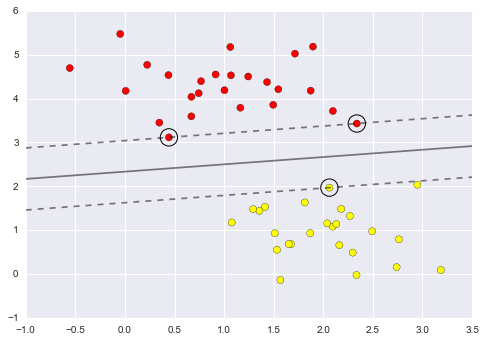
\includegraphics[scale=.7]{Immagini/SVM margine.png} \cite{Data science handbook}
\\

Non è sempre possibile tracciare un iperpiano lineare per separare le categorie,
a volte è necessario aggiungere una dimensione ai dati scalandoli secondo una
funzione di kernel che ci permetta poi di tracciare l'iperpiano. Spesso anche
utilizzando il kernel non esiste un margine netto tra le categorie e ci serve un
modo di permettere un margine meno stringente in cui alcuni dati staranno
all'interno del margine, la rigidità del margine è controllata da un parametro
C, più grande è C più lasso sarà il margine.

\section{Alberi di decisione e foreste casuali}

L'obbiettivo di questo approccio è costruire un albero di decisione ovvero una
serie di decisioni basate sul valore di una caratteristica dei dati che ci porta
a separare i dati nelle corrette categorie. Ogni decisione è quindi composta da
una caratteristica e una soglia, per ogni decisione sceglieremo la soglia che
minimizza un indice di eterogeneità, come l'entropia o l'indice di Gini, e che
quindi separa il più possibile le caratteristiche.

Un problema di questo approccio è che tende a fare overfitting soprattutto se
aumentiamo la profondità dell'albero. Un modo di ovviare a questo problema è
quello di usare le foreste casuali un classificatore che aggrega una serie di
alberi di decisioni prendendo la classificazione più popolare tra questi.
Vengono allenati più alberi di decisione con diversi sottoinsiemi del training
set e la classificazione finale sarà ottenuta prendendo la più popolare tra i
diversi alberi di decisione.

\section{Naive Bayes}

Naive Bayes si basa sull'applicazione del teorema di Bayes:
$$
P(y \mid x_1, \dots, x_n) = \frac{P(y) P(x_1, \dots, x_n \mid y)}
                                 {P(x_1, \dots, x_n)}
$$
considerando $y$ come appartenere a una data categoria e $x_n$ come le
caratteristiche dei nostri dati. Perché il teorema sia corretto è necessario che
le $x_n$ siano tra loro indipendenti, questo non è sempre vero ma in problemi
reali si può tipicamente assumerlo come vero e ottenere comunque buoni
risultati. Possiamo stimare $P(y)$, $P(x_1, \dots, x_n \mid y)$ e
$P(x_1, \dots, x_n)$ dal training set e quindi classificare i nuovi dati come la
categoria a cui è più probabile che appartengono.

\section{K-means}

K-means è l'unico algoritmo non supervisionato usato in questo progetto e si
basa sul dividere il training set in K categorie scegliendo K punti detti
baricentri e assegnando ogni punto alla categoria del baricentro più vicino. La
posizione dei baricentri viene ottimizzata cercando di minimizzare la somma
delle distanze quadratiche tra i dati del training set e il loro baricentro più
vicino. 

Essendo questo un algoritmo non supervisionato non è nota l'associazione tra
baricentro e categoria reale e sarà quindi necessario ristabilire questa
associazione ad esempio associando ogni baricentro alla categoria più presente
nel suo insieme.


% 
% 
%			CAPITOLO 2: Il problema affrontato
\chapter{Il problema affrontato}
\label{cap2}
\section{Descrizione dei dati}
\section{Ambiente software}
\section{Schema delle prove}
\subsection{Repeated hold out}
\subsection{Convalida incrociata}
\subsection{Griglia di ricerca}


% 
% 
%			CAPITOLO 3: Risultati
\chapter{Risultati}
\label{cap3}
\section{Valutazione combinata}

% 
% 
%			CAPITOLO 4: Conclusioni
\chapter{Conclusioni}
\label{cap4}

%
%			BIBLIOGRAFIA
%
\begin{thebibliography}{00}
%
% \bibitem{gotti91}
% M. Gotti, I linguaggi specialistici, Firenze, La Nuova Italia, 1991.
%
\bibitem{Intro to nn}
D. Kriesel, A brief introduction to neural networks, available at
http://www.dkriesel.com, 2007. %Seguendo "how to cite" sul sito
%

% https://towardsdatascience.com/support-vector-machine-introduction-to-machine-learning-algorithms-934a444fca47
\bibitem{Data science handbook}
Jake VanderPlas, Python Data Science Handbook, O'Reilly Media, aviable at
https://jakevdp.github.io/PythonDataScienceHandbook/, 2016


\end{thebibliography}
% 
\end{document}


 
